\documentclass[parskip=half-, 12pt, DIV=15, twoside=semi]{scrbook}
\usepackage[sans, frenchstyle]{kpfonts-otf}
%\usepackage{showframe}
\usepackage{polyglossia}
\setmainlanguage{french}
\usepackage{xcolor}
\usepackage{tabularray}
\usepackage{multicol}
\usepackage{tabularray}
\usepackage{graphicx}
\usepackage{marvosym}
\usepackage{enumitem}
\setlist[enumerate]{label=\textbf{\alph*)}}
\SetEnumitemKey{cols}
{
    before = \begin{multicols}{#1},
    after = \end{multicols}
}
\usepackage[use-files]{xsim}
\xsimsetup{
    path=xsim,
    load-style=mytemplate,
    exercise/template=mytemplate,
}
\begin{document}

\begin{center}
    \begin{huge}
        Chapitre 8 - Distance et lieux 
    \end{huge}
\end{center}

\medbreak

\setcounter{chapter}{8}

\section{Inégalité triangulaire}
Un triangle n'est constructible que si la longueur du plus grand côté est inférieure à la somme des longueurs des deux autres côtés.

Exemples :

\vspace{2cm}

\section{Positions relatives}
\subsection{Positions relatives d'une droite et d'un cercle}

La droite peut être :
\begin{list}{\textbullet}{\itemsep=3cm}
    \item Extérieure au cercle (aucun point de contact)
    \item Tangente au cercle (un seul point de contact, perpendiculaire à un rayon)
    \item Sécante au cercle (deux points de contact)
\end{list}
\vspace{0.5cm}
\newpage

\subsection{Positions relatives de deux cercles}

Deux cercles peuvent être : 
\begin{list}{\textbullet}{\itemsep=3cm}
    \item Concentriques
    \item Disjoints intérieurs
    \item Tangents intérieurs
    \item Sécants
    \item Tangents extérieurs
    \item Disjoints extérieurs
\end{list}
\vspace{1cm}

\newpage
\section{Distances}

\begin{center}
    \begin{tblr}{
            hlines,
            vlines,
            rows={4cm,m},
            row{1}={gray!40, font=\bfseries},
            column{1}={3cm},
            column{2}={4cm},
            column{3}={8cm},
        }
        Par rapport à & On doit tracer & Exemple : le lieu des points se situant  \\
        un point & &  \\
        deux points & & \\
        une droite & & \\
        deux droites & & \\
    \end{tblr}
\end{center}

\section{Cercles inscrits et circonscrits}
\subsection{Cercles inscrits}

À l'intérieur du triangle, tangent aux 3 côtés du triangle

\rightarrow Tracer les \textbf{bissectrices }\\
\begin{center}
    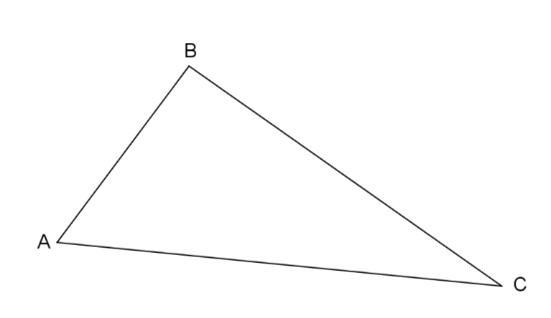
\includegraphics{img/triangleABC.png}
\end{center}

\subsection{Cercles circonscrits}

Qui passe par les 3 sommets du triangle

\rightarrow Tracer les \textbf{médiatrices} \\
\begin{center}
    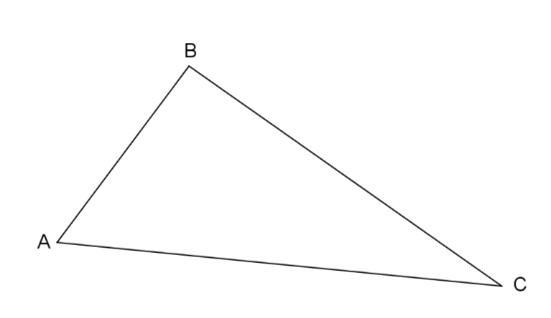
\includegraphics{img/triangleABC.png}
\end{center}

\vfill
\section{Exercices}

Exercices issus de CE1D des années précédentes (pages 152 à 157 du syllabus)
\end{document}